    \section{Challenges : Diffie-Hellman}
    \subsection{Introduction à l'échange de clés Diffie-Hellman}
    Cette catégorie aborde le protocole d'échange de clés de
    Diffie-Hellman, un mécanisme de cryptographie asymétrique.
    Proposé en 1976, il a pour objectif de résoudre le problème de la
    distribution de clés sur un canal de communication non sécurisé.

    Le principe de ce protocole repose sur l'utilisation de fonctions
    mathématiques à sens unique, dont le calcul est aisé dans une direction
    mais calculatoirement difficile à inverser. Spécifiquement, Diffie-Hellman
    s'appuie sur la difficulté du problème du logarithme discret dans
    un groupe fini. Ce procédé permet à deux interlocuteurs d'établir une clé
    secrète partagée sans transmission préalable de celle-ci, y compris en
    présence d'un adversaire observant la communication.

    Les challenges de cette section visent à analyser les fondements
    mathématiques de ce protocole, ainsi que les vulnérabilités pouvant
    résulter d'une implémentation incorrecte ou d'un choix de paramètres
    inadéquat.

    \subsection{L'attaque de l'homme du milieu (\textit{Man-in-the-Middle})}
    Cette sous-partie examine une vulnérabilité du protocole Diffie-Hellman~:
    l'attaque de l'homme du milieu (\textit{Man-in-the-Middle} ou MitM). Le protocole de
    base, dans sa forme originelle, ne fournit aucun mécanisme d'authentification
    des interlocuteurs. Il permet de s'assurer que la clé partagée est secrète,
    mais pas de vérifier l'identité de la personne avec qui on la partage.

    Une attaque MitM exploite cette absence d'authentification. Un adversaire
    se positionne entre les deux communicants, intercepte leurs messages publics
    et établit une session Diffie-Hellman distincte avec chacun d'eux. Chaque
    interlocuteur génère alors une clé secrète partagée avec l'attaquant, tout
    en croyant communiquer directement l'un avec l'autre.

    L'adversaire peut alors déchiffrer les messages, les lire, les modifier, puis
    les rechiffrer avec la clé de l'autre session avant de les transmettre au
    destinataire final. Les challenges de cette section illustrent comment
    cette interception est mise en œuvre et comment elle compromet la
    confidentialité et l'intégrité de l'échange.

    Pour illustrer ce type d'attaque, nous présentons le challenge \textit{Export-Grade}.

    \subsubsection{Objectifs}
    L'objectif de ce challenge est de compromettre la confidentialité d'un
    échange sécurisé par le protocole Diffie-Hellman. Le scénario repose sur
    une attaque de l'homme du milieu (\textit{Man-in-the-Middle}) durant la phase de
    négociation des paramètres cryptographiques.

    La vulnérabilité exploitée est la capacité pour un attaquant d'influencer
    le choix des paramètres de groupe utilisés par les deux correspondants. En
    les contraignant à utiliser un groupe de petite taille (64 bits), le
    problème mathématique du logarithme discret, sur lequel repose la sécurité
    du protocole, devient calculatoirement soluble. La résolution de ce
    problème permet de retrouver une clé privée, et par conséquent la clé
    secrète partagée utilisée pour chiffrer la communication.

    \subsubsection{Méthode}
    Notre attaque s'est déroulée en plusieurs étapes. Premièrement, nous avons
    activement intercepté la communication initiale d'Alice, qui proposait une
    liste de groupes cryptographiques. Nous avons altéré ce message en ne
    conservant que le groupe le plus faible, caractérisé par un module de 64
    bits, avant de le transmettre à Bob. L'acceptation de cette unique option
    par Bob a été relayée à Alice, établissant ainsi un accord sur un canal de
    communication affaibli.

        \begin{figure}[H]
            \centering
            % La commande pour insérer l'image.
            % 'width=0.8\linewidth' signifie que l'image fera 80% de la largeur du
            % texte.
            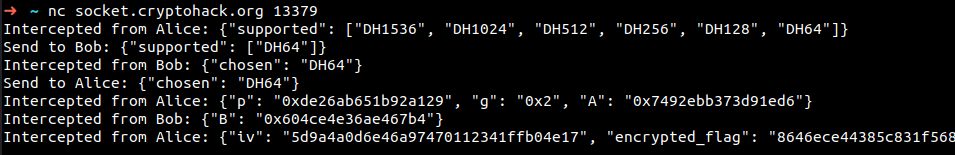
\includegraphics[width=0.95\linewidth]{Images/DiffieHellman/capture_mitm.png}

            % La légende qui apparaîtra sous l'image.
            \caption{Capture d'écran de la communication interceptée entre Alice et Bob en tant que \textit{Man-In-The-Middle}.}

            % L'étiquette pour y faire référence plus tard.
            \label{fig:mitmChallenge}
        \end{figure}

    Une fois cet accord forcé, notre rôle est devenu passif. Nous avons
    collecté les paramètres publics de l'échange : le module \textit{p}, le
    générateur \textit{g}, et les clés publiques d'Alice (\textit{A}) et de
    Bob (\textit{B}). La faible taille du module \textit{p} a alors permis de
    résoudre le problème du logarithme discret. L'échange réalisé avec Alice et Bob est illustré \hyperref[fig:mitmChallenge]{Figure 5}. 
    
    À l'aide d'un script Python, nous
    avons calculé la clé privée \textit{a} d'Alice à partir des valeurs publiques
    \textit{p}, \textit{g} et \textit{A}. La connaissance de cette clé privée nous a permis de reconstituer la clé
    secrète partagée ($s = B^a \pmod{p}$). Cette dernière a servi à dériver la
    clé de session AES, avec laquelle nous avons déchiffré le message final
    pour obtenir le \textit{flag}.

    \subsubsection{Résultat}
    L'attaque par manipulation des paramètres a réussi. En forçant l'usage d'un
    groupe faible, nous avons pu calculer la clé privée, reconstituer la clé de
    session et déchiffrer le message, révélant le \textit{flag} suivant :

    \begin{center}
        \texttt{crypto\{d0wn6r4d35\_4r3\_d4n63r0u5\}}
    \end{center}

    Le script développé pour la résolution du challenge est présenté \hyperref[annexe:script-exportgrade]{Annexe E}.

    \subsection{Théorie des groupes}
    Cette sous-partie aborde les structures mathématiques qui sous-tendent de
    nombreux protocoles de cryptographie asymétrique~: les groupes. En
    algèbre abstraite, un groupe est un ensemble d'éléments muni d'une
    opération binaire qui satisfait à des axiomes spécifiques (fermeture,
    associativité, existence d'un élément neutre et d'un inverse pour chaque
    élément).

    La sécurité de protocoles comme Diffie-Hellman ne repose pas sur les
    nombres en tant que tels, mais sur les propriétés structurelles de ces
    groupes mathématiques. Des concepts comme l'ordre d'un groupe, l'ordre
    d'un élément, et la notion de générateur d'un groupe
    cyclique sont des composantes directes de l'implémentation et de
    l'analyse de sécurité de ces systèmes.

    Les challenges de cette section ont pour objectif d'étudier ces
    propriétés. Ils illustrent comment les caractéristiques d'un groupe, ou le
    choix de ses paramètres, peuvent influencer la robustesse d'un schéma
    cryptographique.

    Pour illustrer cette section, nous présentons le challenge \textit{Additive}.

    \subsubsection{Objectifs}
    \begin{sloppypar}
    L'objectif de ce challenge est de calculer une clé secrète partagée dans une
    implémentation du protocole Diffie-Hellman utilisant un groupe additif.
    Contrairement à l'implémentation classique qui utilise un groupe
    multiplicatif d'entiers modulo un nombre premier, ce challenge transpose le
    problème dans une structure où l'opération de groupe est l'addition.
    \end{sloppypar}

    Le principe de sécurité reste fondé sur la difficulté d'inverser une
    fonction à sens unique. Ici, l'opération équivalente à l'exponentiation est
    la multiplication scalaire. Le but est de résoudre l'équivalent du problème
    du logarithme discret dans ce contexte additif afin de retrouver une clé
    privée, puis de reconstituer la clé secrète partagée, qui constitue le
    \textit{flag}.

    \subsubsection{Méthode}
    Le challenge nous fournit les paramètres publics d'un échange
    Diffie-Hellman additif : un module premier \textit{p}, un générateur
    \textit{g}, ainsi que les clés publiques d'Alice (\textit{A}) et de Bob
    (\textit{B}). La relation qui lie la clé privée \textit{a} à la clé
    publique \texttt{A} n'est plus $A = g^a \pmod{p}$, mais
    $A = a \cdot g \pmod{p}$.

    Le problème du logarithme discret se traduit ici par la résolution de
    l'équation $A \equiv a \cdot g \pmod{p}$ pour trouver l'inconnue
    \textit{a}. Cette équation est une congruence linéaire qui se résout
    efficacement en calculant l'inverse modulaire de \textit{g} modulo
    \textit{p}. Nous avons donc déterminé la clé privée d'Alice en calculant
    $a = A \cdot g^{-1} \pmod{p}$.

    Une fois la clé privée \textit{a} obtenue, nous avons pu calculer la clé
    secrète partagée en appliquant l'opération du groupe avec la clé publique
    de Bob. L'opération étant la multiplication scalaire, la clé secrète
    \textit{s} est obtenue par la formule $s = a \cdot B \pmod{p}$.

    \subsubsection{Résultat}
    L'analyse de la structure de groupe additive a permis d'identifier la
    méthode de résolution appropriée. Le calcul de l'inverse modulaire nous a
    donné accès à la clé privée, menant directement à la reconstitution de la
    clé secrète partagée. Nous avons obtenu le \textit{flag} suivant :

    \begin{center}
        \texttt{crypto\{cycl1c\_6r0up\_und3r\_4dd1710n?\}}
    \end{center}
